\newpage
\noindent
\section{Auswertung}
    \subsection{Statische Methode}
        Bei der statischen Methode wird jeweils an zwei Stellen eines jeden Metallstabes die Temperatur als Funktion der Zeit gemessen und über den zeitlichen
        Temperaturverlauf wird an den beiden Messstellen die Wärmeleitfähigkeit der vier Metallstäbe bestimmt.

        \subsubsection{Temperaturverläufe der fernen Thermoelemente}
        Im folgenden befindet sich eine Grafik für alle fernen Thermoelemente. Dabei misst das Thermoelement $T1$ an dem dicken Messingstück und $T4$ am dünnen. $T5$ und $T8$ sind
        jeweils am Aluminium und Edelstahl befestigt.

        \begin{figure}
               \centering
               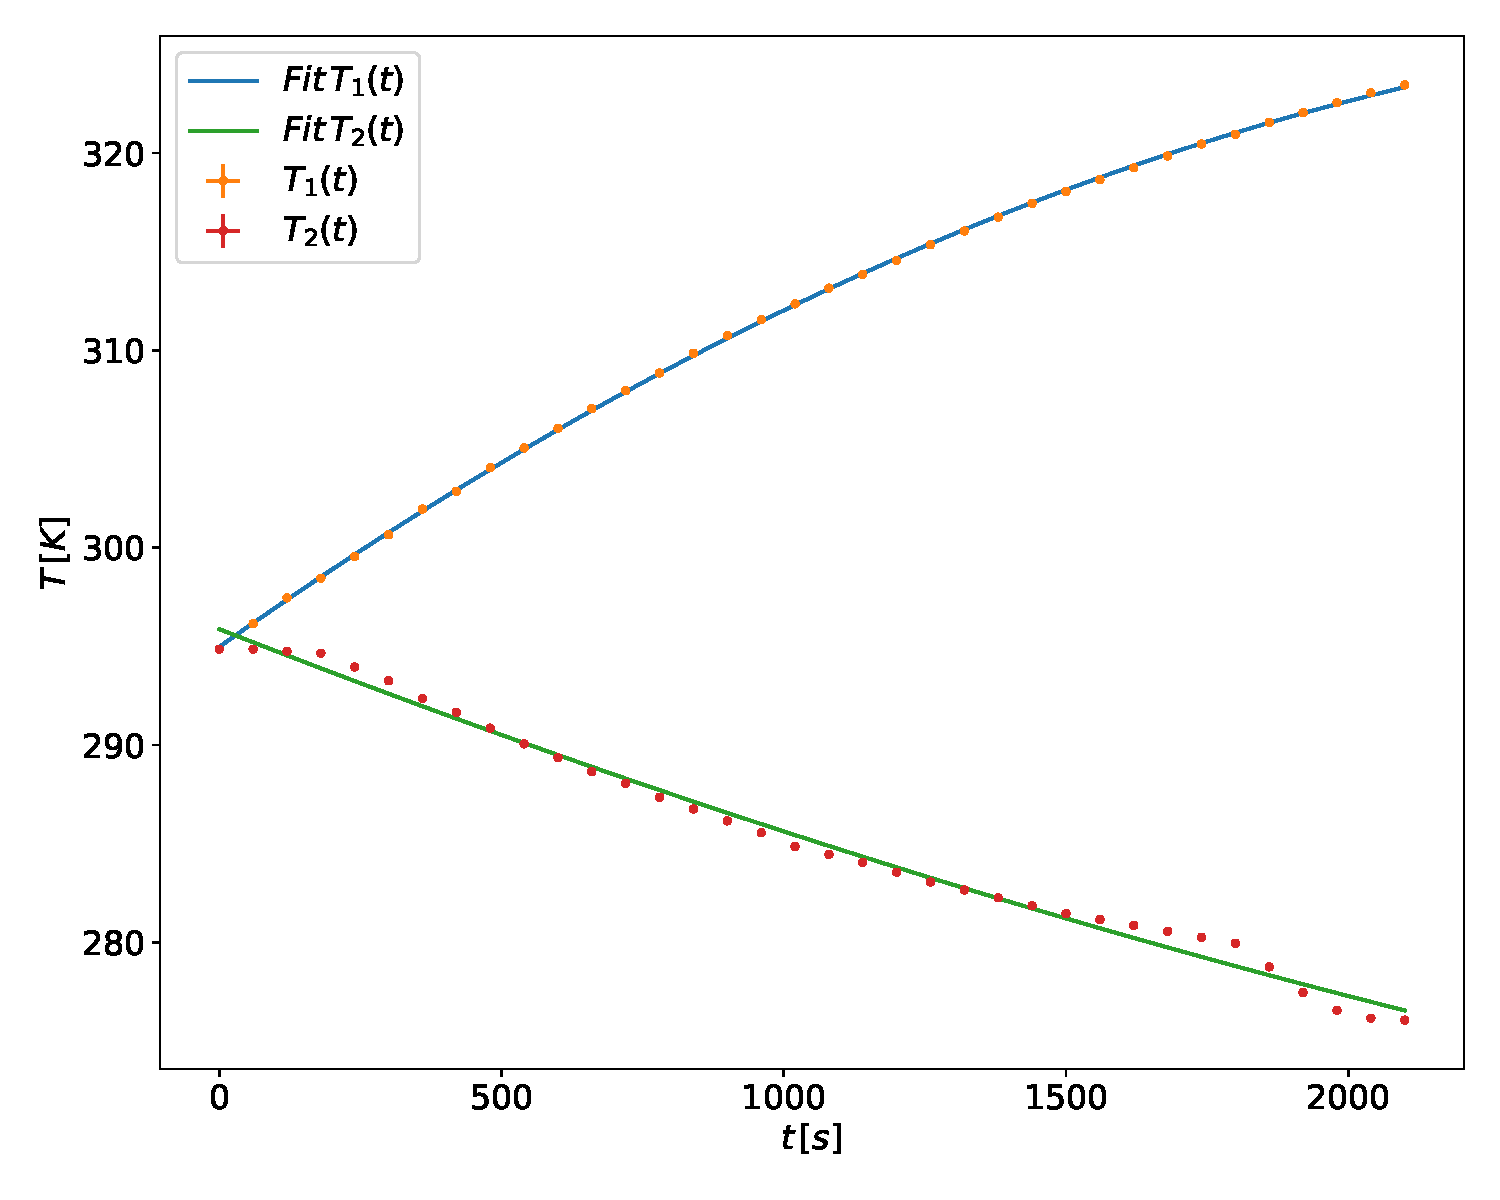
\includegraphics[width=\textwidth]{Daten/grafic.pdf}
               \caption{Temperaturverläufe der fernen Thermoelemente $T1$, $T4$, $T5$, $T8$}
               \label{fig:static_far}
        \end{figure}
\noindent
        Es fällt auf, dass $T1$ und $T4$ ungefähr von $t = 0 \si{\second}$ bis $t = 100 \si{\second}$ gleichstark steigen, jedoch steigt die Temperatur von $T5$ deutlich steiler und von $T8$ deutlich 
        flacher als die gemessene Temperatur der anderen Thermoelemente.
        Zudem ist bei allen Thermoelementen, außer bei $T8$, ab $t = 600 \si{\second}$ ein starker Knick zu beobachten. Außerdem steigt $T8$ nicht sofort, sowie die anderen Kurven direkt, sondern verzögert. 
        Es ist außerdem auffällig das alle Kurven nach dem Abflachen nahezu parallel verlaufen.

\noindent
        An den Graphen lässt sich jeweils die Temperaturen bei 700s ablesen.
        \begin{align*}
         T1(700 \si{\second}) &=  318.06 \, \si{\kelvin} = 44.91 \, \si{\celsius}\\ 
         T4(700 \si{\second}) &=  316.42 \, \si{\kelvin} = 43.27 \, \si{\celsius}\\
         T5(700 \si{\second}) &=  320.66 \, \si{\kelvin} = 47.51 \, \si{\celsius}\\
         T8(700 \si{\second}) &=  318.06 \, \si{\kelvin} = 44.91 \, \si{\celsius}
        \end{align*}
\noindent
        Aus der Grafik lässt sich erkennen, dass die Temperatur von T5 bei 700s am größten ist. Daraus lässt sich schlussfolgern, dass die Wärmeleitfähigfkeit von Aluminium im Vergleich zu Edelstahl und Messing am besten ist.

        \subsubsection{Wärmestrom}
        Mit der Gleichung (\ref{eqn:waermemenge}) lässt sich nach einer Umstellung zu $\frac{\symup{d}Q}{\symup{d}t} $ der Wärmstrom als differenz $\frac{\Delta Q}{\Delta t} = s $ berechnen. 
        Diese werden in der folgenden Tabelle bei den unterschiedlichen Materialien jeweils bei $t = {0\si{\second},100\si{\second},200\si{\second},300\si{\second},400\si{\second},500} \si{\second}$ bestimmt:

        
        \begin{table}
        \centering
            \begin{tabular}{
                S[table-format=3.0]
                S[table-format=1.3]
                S[table-format=1.3]   
                S[table-format=1.3]
                S[table-format=1.3]
            }
            \toprule
            {$t \mathbin{/} \si{\second} $} 
            & {$s_\text{Messing(Dick)}  \mathbin{/} \si[per-mode=fraction]{\kilo\gram\square\meter\per\second\cubic} $}
            & {$s_\text{Messing(Dünn)}  \mathbin{/} \si[per-mode=fraction]{\kilo\gram\square\meter\per\second\cubic} $}
            & {$s_\text{Aluminium}      \mathbin{/} \si[per-mode=fraction]{\kilo\gram\square\meter\per\second\cubic} $}
            & {$s_\text{Edelstahl}      \mathbin{/} \si[per-mode=fraction]{\kilo\gram\square\meter\per\second\cubic} $} \\
            \midrule
            0   & 0.038 & -0.052 & 0.011 & -0.018 \\
            100 & 0.917 & -0.569 & 0.700 & -0.346 \\
            200 & 0.634 & -0.420 & 0.474 & -0.300 \\
            300 & 0.566 & -0.387 & 0.435 & -0.272 \\
            400 & 0.552 & -0.377 & 0.431 & -0.259 \\
            \bottomrule
            \end{tabular}
        \caption{Messdaten}
        \label{tab:5_Mess}
        \end{table}
\newpage
        \subsection{Diagramme der Temperaturdifferenzen}
    \noindent
    Im folgenden sínd 2 Diagramme dargestellt. Bei beiden wird die Temperaturdifferenzen der Termoelemente eines Werkstückes gegen die Zeit aufgetragen. Bei dem linken Diagramm handelt es sich um das Edelstahl und beim rechten um die Temperaturdifferenz beim dicken Messingstück.
    \begin{figure}
        \begin{subfigure}{0.48\textwidth}
               \centering
               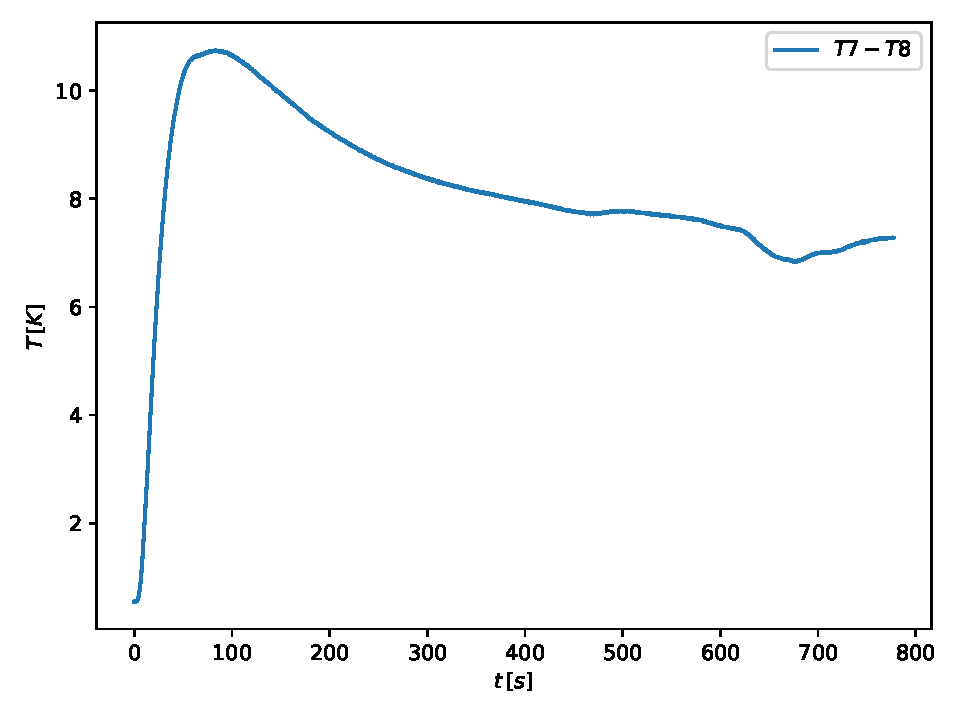
\includegraphics[height=5.5cm]{Daten/grafic1.pdf}
               \caption{Temperaturverlauf von $T7-T8$}
               \label{fig:static_T7-T8}
        \end{subfigure}
    \hfill
        \begin{subfigure}{0.48\textwidth}
               \centering
               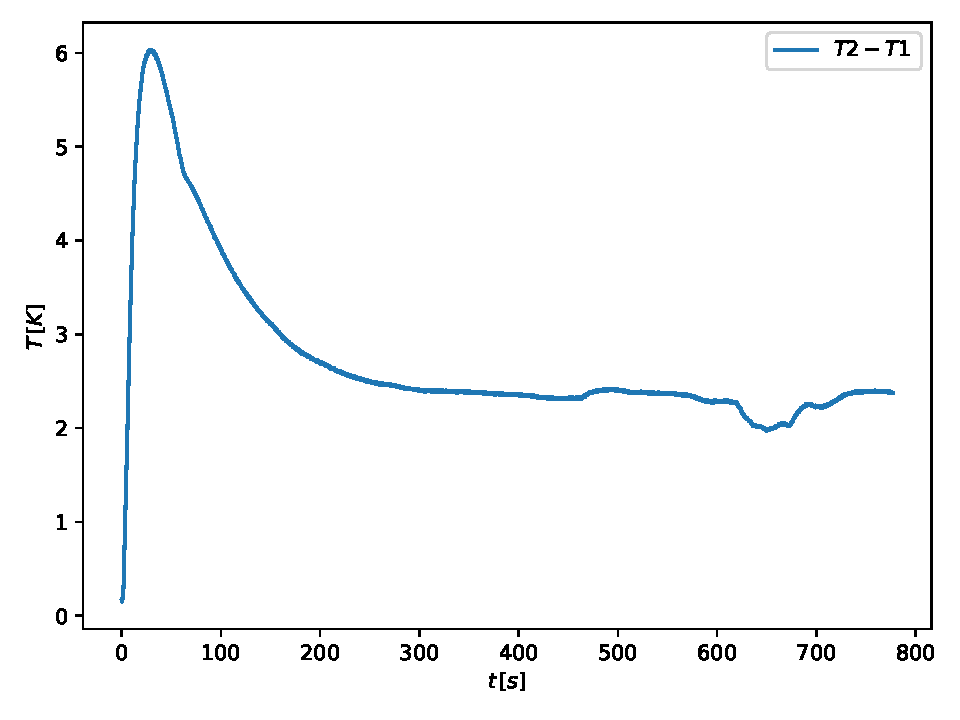
\includegraphics[height=5.5cm]{Daten/grafic2.pdf}
               \caption{Temperaturverlauf von $T2-T1$}
               \label{fig:static_T2-T1}
        \end{subfigure}
    \end{figure}
\noindent
    Es fällt auf das beide Graphen mit einer ungefähr gleichen Steigung steigen. Zudem flachen beide Graphen bei großem t relativ stark ab und haben beide eine \glqq Kuhle \grqq{} ab ungefähr t=630s.
    Außerdem haben beide einen Hochpunkt bei ungefähr t=50s. 
\noindent
Jedoch fällt der Graph von $T2-T1$ deutlich stärker als $T7-T8$. Das globale Maximum von $T7-T8$ liegt ebenfalls höher, als $T2-T1$. Bei genaueren hinschauen wird bei den beiden Globalen Maxima,
    erkannt, dass das Messing vor dem Edelstahl sein Maximum annimmt. 
\noindent
    Der geringe Abfall von $T7-T8$ und der hohe Graph, sowie das höhere Maxima deutet darauf hin, dass die Wärmeleitfähigkeit von Edelstahl signifikant schlechter ist als von Messing. Dies lässt sich auch in den
    errechneten Wärmeleitfähigkeiten sehen.
\newpage
    \subsection{Dynamische Methode mit einer 80s Periode}

    Im folgenden sind die beiden Temperaturverläufe für den breiten Messingstab (T1 und T2), bei einem Umschalten von 'HEAT' auf 'COOL' alle 40s, graphisch dargestellt.

    %Messing
    \subsubsection{Messing}

    \begin{figure}
    \centering
    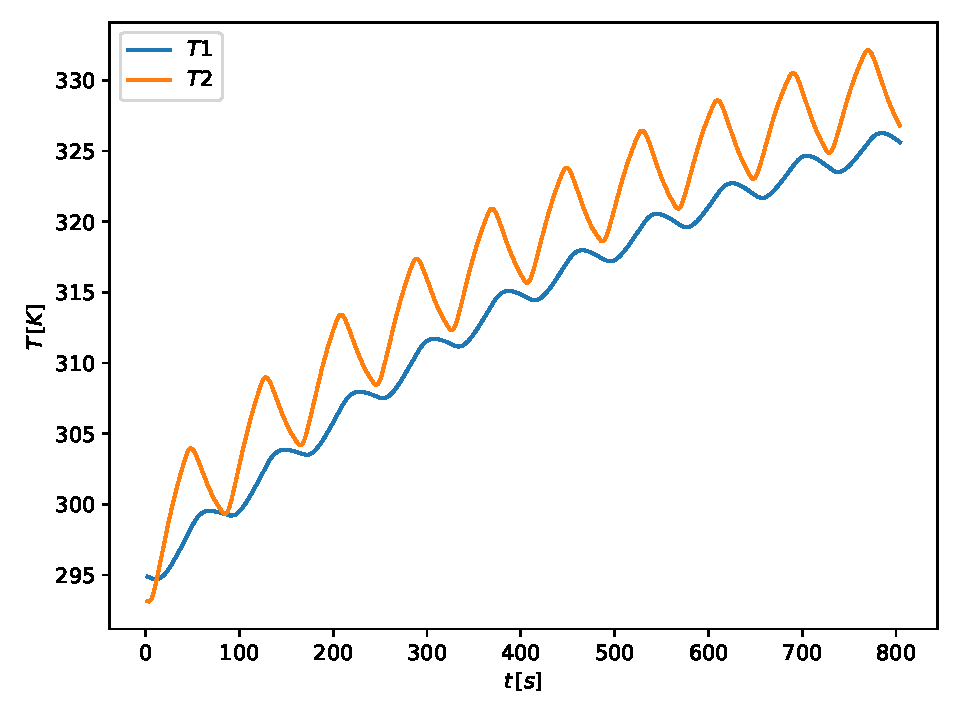
\includegraphics[width=\textwidth]{Daten/grafic3.pdf}
    \caption{Temperaturverlauf von $T1$ und $T2$}
    \label{fig:dyn_T1}
    \end{figure}
    \noindent
    Aus der Grafik lassen sich die doppelten Amplituden $A1 \, \text{und} \, A2$ sowie die Phasendifferenz $\Delta t$ bestimmen. Daraus lässt sich die dazugehörige Wärmeleitfähigkeit berechnen:
    \begin{table}
        \centering
            \begin{tabular}{
                S[table-format=1.3]
                S[table-format=2.2]
                S[table-format=2.0]
                S[table-format=3.2]
            }
            \toprule
            {$ {A1}         \mathbin{/} \si[per-mode=fraction]{\kelvin} $}
            & {$ {A2}       \mathbin{/} \si[per-mode=fraction]{\kelvin} $}
            & {$\Delta t \mathbin{/} \si[per-mode=fraction]{\second} $}
            & {$\kappa   \mathbin{/} \si[per-mode=fraction]{\watt\per\meter\per\kelvin}$} \\
            \midrule
            4.85 & 10.86 & 13. & 127.07  \\
            4.66 &  9.68 & 13. & 140.12 \\
            4.46 &  9.27 & 13. & 140.01 \\
            4.21 &  8.95 & 14. & 126.12 \\
            3.93 &  8.61 & 12. & 141.50 \\
            3.54 &  8.14 & 12. & 133.27 \\
            3.36 &  7.84 & 12. & 130.97 \\
            3.12 &  7.69 & 11. & 134.20 \\
            2.97 &  7.53 & 11. & 130.12 \\
            2.77 &  7.28 & 12. & 114.84 \\
            \bottomrule
            \end{tabular}
        \caption{Errechnete Daten fürs Messing aus dem Graphen}
        \label{tab:MesMess}
    \end{table}
    \noindent
    Es fällt auf das diese stark schwankt, jedoch ist nach einer Mittelung der Werte der Fehler zum Literaturwert aus (\ref{tab:literaturwerte}) nicht mehr so groß.

    %Aluminium
\newpage
    \subsubsection{Aluminium}
    \begin{figure}
    \centering
    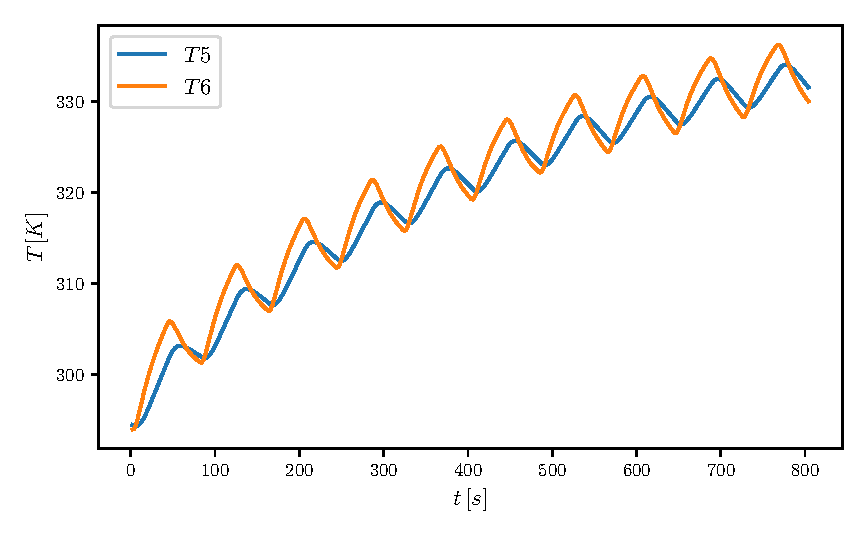
\includegraphics[width=\textwidth]{Daten/grafic5.pdf}
    \caption{Temperaturverlauf von $T5$ und $T6$}
    \label{fig:dyn_T5}
    \end{figure}
\noindent
    Um die Rechnung zu vereinfachen wurden die Werte, welche aus dem Diagramm wie bereits beim Messing bestimmt wurden, direkt als Mittelwerte berchnet. Diese sind in der folgenden Tabelle dargestellt:
    \begin{table}
        \centering
            \begin{tabular}{
                S[table-format=1.3]
                S[table-format=1.3]
                S[table-format=2.3]
                S[table-format=3.3]
            }
            \toprule
            {$ {A5}         \mathbin{/} \si[per-mode=fraction]{\kelvin} $}
            & {$ {A6}       \mathbin{/} \si[per-mode=fraction]{\kelvin} $}
            & {$\Delta t \mathbin{/} \si[per-mode=fraction]{\second} $}
            & {$\kappa   \mathbin{/} \si[per-mode=fraction]{\watt\per\meter\per\kelvin}$} \\
            \midrule
            6.477 & 5.497 & 32.889 & 201.702  \\
            \bottomrule
            \end{tabular}
        \caption{Errechnete Daten fürs Aluminium aus dem Graphen}
        \label{tab:MesAlu}
    \end{table}
\noindent
    Auch hier sieht man eine kleine Abweichung zum Literaturwert. Diese Abweichungen sind in der Diskussion diskutiert.


\noindent
\newpage
\subsubsection{Wellenlänge und Frequenz bei Messing und Aluminium}
    Zusätzlich kann man die Frequenz, sowie die Wellenlänge aus den Daten berechnen. Die Frequenz der Welle im Messing und Aluminium wird aus der Grafik (\ref{fig:dyn_T1}) und (\ref{fig:dyn_T5}) bestimmt, indem die Anzahl der Perioden durch das gewählte Intervall geteilt wird.
    Dies für dann zu den folgenden Werten:
    % Tabelle für Wellenlänge von Messing
    \begin{table}
        \centering
            \begin{tabular}{c c c c}
            \toprule
            {$   f_1 \mathbin{/}\si{\hertz} $}
            & {$ f_2 \mathbin{/} \si{\hertz} $}
            & {$ f_5 \mathbin{/} \si{\hertz} $}
            & {$ f_6 \mathbin{/} \si{\hertz} $} \\
            \midrule
            0.01228 & 0.01277 & 0.0125 & 0.0125\\
            \bottomrule
            \end{tabular}
        \caption{Frequenz aus den Graphen ermittelt}
        \label{tab:MesWelle}
    \end{table}

\noindent  
    Daraus lässt sich Mithilfe der Formel $\lambda f = \upsilon$ und der Formel (\ref{eqn:phasengeschwindigkeit}) die Frequenz berechnen zu:
\begin{table}
        \centering
            \begin{tabular}{c c c c}
            \toprule
            {$   \lambda_1 \mathbin{/} \si{\meter} $}
            & {$ \lambda_2 \mathbin{/} \si{\meter} $}
            & {$ \lambda_5 \mathbin{/} \si{\meter} $}
            & {$ \lambda_6 \mathbin{/} \si{\meter} $} \\
            \midrule
            0.00256 & 0.00261 & 0.00379 & 0.00379\\
            \bottomrule
            \end{tabular}
        \caption{Wellenlänge errechnet}
        \label{tab:MesWelle}
    \end{table}


    \subsection{Dynamische Methode mit einer 200s Periode}
    
\noindent
    Die selbe Auswertung die bei Aluminium und Messing erfolgte, erfolgt jetzt ebenfalls bei Edelstahl, bei welchem ein Umschalten von 'HEAT' auf 'COOL' alle 100s erfolgt. Jedoch wurde diesmal von vielen Perioden die Amplitude bestimmt und jeweils die Wärmeleitfähigfkeit $\kappa$ ausgerechnet und nicht nur leidglich mit der gemittleten Amplitude.
    
    \begin{figure}
               \centering
               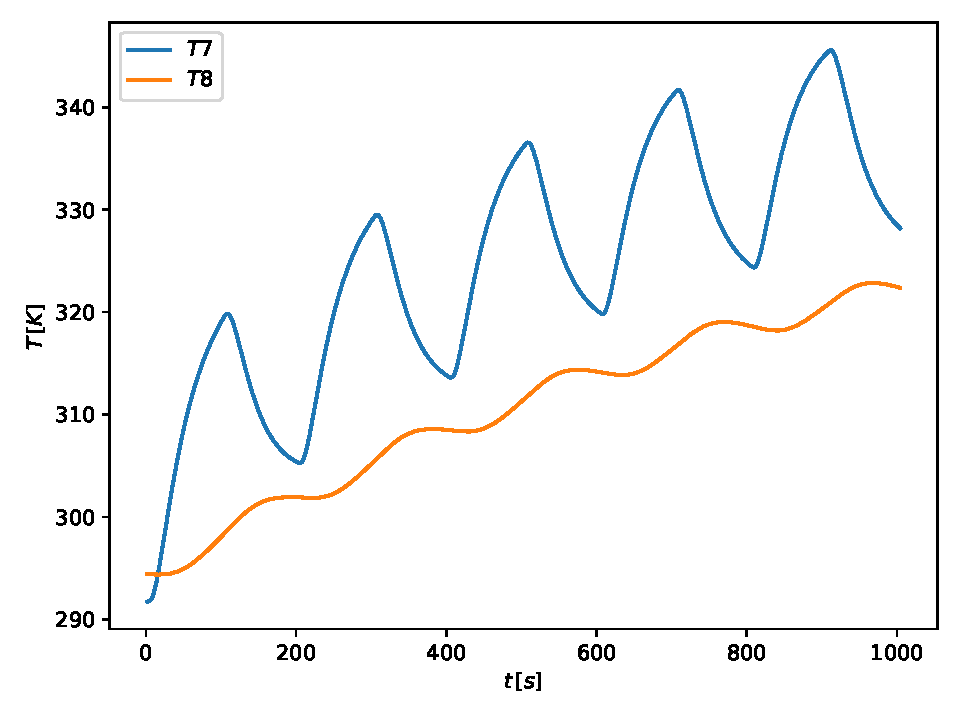
\includegraphics[width=\textwidth]{Daten/grafic4.pdf}
               \caption{Temperaturverläufe der Thermoelemente $T7$ und $T8$}
               \label{fig:dyn_edel}
        \end{figure}

    \begin{table}
        \centering
            \begin{tabular}{
                S[table-format=2.0]
                S[table-format=2.0]
                S[table-format=1.2]   
                S[table-format=2.3]
            }
            \toprule
            {$A7_\text{Edelstahl} \si{\kelvin} $}
            & {$A8_\text{Edelstahl} \si{\kelvin} $}
            & {$\Delta t_\text{Edelstahl} \si{\second} $}
            & {$\kappa_\text{Edelstahl} \si[per-mode=fraction]{\watt\per\meter\per\kelvin} $}\\
            \midrule
            14.59 & 0.07   & 48 & 7.659 \\
            15.92 & 0.25   & 48 & 9.845 \\
            16.74 & 0.53   & 47 & 11.844\\
            17.32 & 0.86   & 45 & 13.619\\
            \bottomrule
            \end{tabular}
        \caption{Errechnete Daten aus den Graphen}
        \label{tab:MesAlum}
    \end{table}
\newpage
    \subsection{Wellenlänge und Frequenz beim Edelstahl}
    Auch beim Edelstahl ist es möglich die Frequenz aus dem Graphen zu bestimmen und im selben Verfahren wie zuvor die Wellenlänge rechnerisch zu bestimmen:
\begin{table}
        \centering
            \begin{tabular}{c c}
            \toprule
            {$ f_7 \mathbin{/} \si{\hertz} $}
            & {$ f_8 \mathbin{/} \si{\hertz} $} \\
            \midrule
            0.004918 & 0.005172 \\
            \bottomrule
            \end{tabular}
        \caption{Frequenz aus den Graphen ermittelt}
        \label{tab:MesWellen}
    \end{table}

    Daraus lässt sich Mithilfe der Formel $\lambda f = \upsilon$ und der Formel (\ref{eqn:phasengeschwindigkeit}) die Frequenz berechnen zu:
\begin{table}
        \centering
            \begin{tabular}{c c}
            \toprule
            {$   \lambda_7 \mathbin{/} \si{\meter} $}
            & {$ \lambda_8 \mathbin{/} \si{\meter} $} \\
            \midrule
            0.00057 & 0.00058 \\
            \bottomrule
            \end{tabular}
        \caption{Wellenlänge errechnet}
        \label{tab:MesWellene}
    \end{table}